% Copyright (C) 2005-2015 Airbus - EDF - IMACS - Phimeca
% Permission is granted to copy, distribute and/or modify this document
% under the terms of the GNU Free Documentation License, Version 1.2
% or any later version published by the Free Software Foundation;
% with no Invariant Sections, no Front-Cover Texts, and no Back-Cover
% Texts.  A copy of the license is included in the section entitled "GNU
% Free Documentation License".
\renewcommand{\filename}{docUC_InputWithData_FittingTests.tex}
\renewcommand{\filetitle}{UC : Distribution fitting tests, numerical and visual validation tests : Chi-squared test, Kolmogorov test, QQ-plot graph}

% \HeaderNNIILevel
% \HeaderIILevel
\HeaderIIILevel



\index{Graph!QQ-plot}
\index{Fitting Test!QQ-plot}
\index{Fitting Test!ChiSquared}
\index{Fitting Test!Kolmogorov}
\index{Fitting Distribution!Parametric method}



The objective of this Use Case is to :
\begin{itemize}
\item perform some parametric fitting tests on a numerical sample in dimension 1, with the maximum likelihood principle or the moment based method,
\item validate these estimations with numerical tests : the Kolmogorov test (continuous distributions) or the Chi -squared test (discrete distributions),
\item validate these estimations with a visual test : the QQ-plot graph.
\end{itemize}

The QQ-plot visual validation test is used with a numerical sample (representing the data) and a distribution (representing the fitted one). For each point of the numerical sample used in the graph, Open Turns evaluates its empirical quantile and associates to it the corresponding quantile from the fitted distribution. \\

Details on the Maximum Likelihood  Principle may be found in the Reference Guide (\extref{ReferenceGuide}{see files Reference Guide - Step B -- Maximum Likelihood  Principle}{stepB}).\\

Details on the Parametric estimators used to evaluate the parameters of the copula may be found in the Reference Guide (\extref{ReferenceGuide}{see files Reference Guide - Step B --  Parametric Estimation}{stepB}).\\

Details on the QQ-polt, Kolmogorov-Smirnov and  Chi-squared tests may be found in the Reference Guide (\extref{ReferenceGuide}{see files Reference Guide - Step B --  Graphical goodness-of-fit tests : QQ-plot and Henry line and Step B -- Kolmogorov-Smirnov goodness-of-fit test}{stepB}).\\


The example here presents :
\begin{itemize}
\item the fitting of a numerical sample of dimension 1 with a Beta distribution, its validation with the Kolmogorov test and the  QQ-Plot graph,
\item the fitting of a numerical sample of dimension 1 with a Poisson distribution, its validation with the Chi-squared test and the  QQ-Plot graph.
\end{itemize}


\requirements{
  \begin{description}
  \item[$\bullet$] a scalar numerical sample (data) : {\itshape sample}
  \item[type:]  NumericalSample
  \end{description}
}
             {
               \begin{description}
               \item[$\bullet$] a Beta and Geometric estimated  distribution : {\itshape estimatedBeta, estimatedGeom}
               \item[type:] Beta, Geometric
               \end{description}

               \begin{description}
               \item[$\bullet$]  results of fitting test : {\itshape resultKolmogorov, resultChiSquared}
               \item[type:] Testresult
               \end{description}
             }

             \textspace\\
             Python script for this UseCase :

             \inputscript{script_docUC_InputWithData_FittingTests}

             \textspace\\


             Figures \ref{qqplotExRight} and \ref{qqplotExFalse} show a QQ-Plot graph to test the adequation of a sample generated  from a Beta(r = 1.2, t = 3.4, a = 1.0, b = 2.0) to :
             \begin{itemize}
             \item the Beta(r = 1.2, t = 3.4, a = 1.0, b = 2.0) distribution : visual validation of the fitting,
             \item the Weibull($\mu$ = 1.5, $\sigma$ = 1.0, $\gamma$ = 1.0) : visual invalidation of the fitting.
             \end{itemize}




             \begin{figure}[H]
               \begin{center}
                 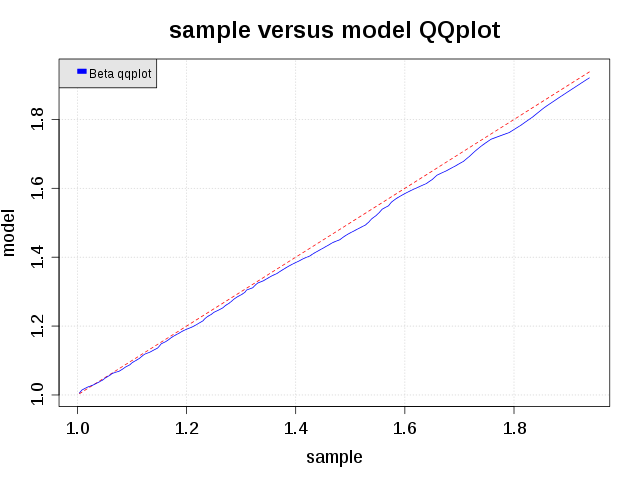
\includegraphics[width=10cm]{Figures/beta_QQplot.png}
               \end{center}
               \caption{Fitting validation by the QQ-Plot graph : Beta fitting to a Beta-sample.}
               \label{qqplotExRight}
             \end{figure}

             \begin{figure}[H]
               \begin{center}
                 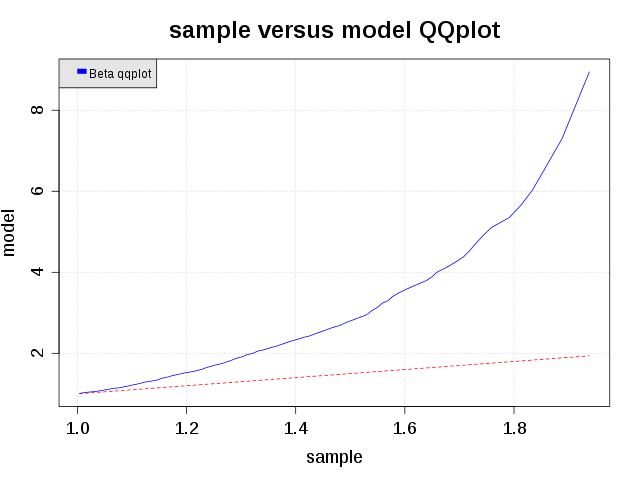
\includegraphics[width=10cm]{Figures/weibull_QQplot.png}
               \end{center}
               \caption{Fitting invalidation by the QQ-Plot graph : Weibull fitting to a Beta sample.}
               \label{qqplotExFalse}
             \end{figure}
